\chapter{Selection}
    \section{Potential Outcomes Framework}
        \subsection{Potential outcome}
            When thinking about the possible effect of a treatment, we need to understand the concept of \textit{potential outcomes}. Inherently, each individual has two \textit{potential outcomes} as defined below.
            \begin{definition}[Potential outcome]
                The \textit{potential outcomes} of $Y_i$ represent the underlying outcomes that would occur if treated or not treated,
                \begin{align}
                    \text{potential outcomes of } Y_i=\begin{cases}
                        Y_{1i}  &\text{"outcome if treated"}   \\
                        Y_{0i}  &\text{"outcome if not treated"}
                    \end{cases}
                \end{align}
            \end{definition}

        \subsection{Observed outcome}
            In reality, we can only actually observe one of the potential outcomes. Let $D_i$ track whether a individual $i$ is treated or not; $D_i = 1$ denotes treated, while $D_i = 0$ means untreated. $D_i$ is an example of what we call a \textit{dummy variable}. 
            \begin{definition}[Observed outcome]
                The \textit{observed outcome} of $Y_i$, simply denoted by $Y_i$, depends on $D_i$ through
                \begin{align}
                    \text{observed outcome, } Y_i &=
                    \begin{cases}
                        Y_{1i}  &\text{if }D_i=1\\
                        Y_{0i}  &\text{if }D_i=0
                    \end{cases}
                \end{align}
                or alternatively, $Y_i = Y_{0i}+D_i\,(Y_{1i}-Y_{0i})$.
            \end{definition}

            In addition, the opposite of the observed outcome is termed the \textit{counterfactual outcome}, i.e. the outcome not observed. For example, if $D_i = 1$ we therefore observe $Y_i = Y_{1i}$, and so $Y_{0i}$ is the counterfactual outcome. The meaning in full can be expressed as
            \begin{quote}
                `The result if individual $i$ (who had actually been treated), had not received treatment'
            \end{quote}

        \subsection{Treatment effects}
            For an individual, the true effect of treatment is $Y_{1i} - Y_{0i}$; but as we discussed above, we can virtually never observe this. In addition, treatment effects may vary from individual to individual. Therefore when analysing experimental results, we would like to understand the effect of treatment on aggregate, defined as ATE below. This is not always possible, and so there are some other similar intuitive concepts defined below:
            \begin{definition}[Average treatment effects]
                We consider three types of average treatment effects.
                \begin{enumerate}
                    \item Average Treatment Effect, ATE $:= \expect{Y_{1i} - Y_{0i}}$
                    \item Average Treatment Effect on the Treated, ATT $:= \expect{Y_{1i} - Y_{0i}| D_i = 1}$
                    \item Average Treatment Effect on the Untreated, ATU $:= \expect{Y_{1i} - Y_{0i}| D_i = 0}$
                \end{enumerate}
            \end{definition}


    \section{The selection problem}
        For us econometricians, we would ideally like to infer the treatment effect for all $i$, $Y_{1i}-Y_{0i}$ or at least the expectation, $\expect{Y_{1i}-Y_{0i}}$. However for an individual, we can’t observe both $Y_{1i}$ and $Y_{0i}$ — depending on the treatment, one must be counterfactual, as discussed above. This is the basic premise of the \textit{selection problem}.

        Before we attempt to tackle this problem, we briefly summarise the quantities that we do actually have:
        \begin{itemize}
            \item $\expect{Y_{1i}|D_i = 1}$ – treatment outcome (for those treated)
            \item $\expect{Y_{0i}|D_i = 0}$ - untreated outcome (for those not treated)
        \end{itemize}
        Based on this, we define the \textit{observed difference} below.
        \begin{definition}[Observed difference]
            The \textit{observed/naïve difference} is defined as
            \begin{align}
                \text{observed difference} := \expect{Y_{1i}|D_i = 1} - \expect{Y_{0i}|D_i = 0}
            \end{align}
            It is the difference in outcomes between the treated group and the untreated group.
        \end{definition}


        \subsection{Selection bias}
            Even without treatment, those who were supposed to be treated may see a difference with the outcome of those who did not receive treatment; this is the idea behind selection bias.

            \begin{definition}[Selection bias]
                \textit{Selection bias} is the difference in untreated outcomes between treatment and untreated groups, defined by
                \begin{align}
                    \text{selection bias} := \expect{Y_{0i}|D_i = 1} - \expect{Y_{0i}|D_i = 0}
                \end{align}
                It represents the inherent baseline difference between the two groups. Note this is not directly observed as the first term is counterfactual.
            \end{definition}

            An important property of the observed difference is discussed in the following theorem:
            \begin{theorem}
                The observed difference can be decomposed into
                \begin{align}
                    \mathrm{observed}\text{ }\mathrm{difference} = \mathrm{ATT} + \mathrm{selection}\text{ }\mathrm{bias}
                \end{align}
            \end{theorem}
            \begin{proof}
                We have
                \begin{align*}
                    \text{observed difference}
                        &:= \expect{Y_{1i}|D_i=1} - \expect{Y_{0i}|D_i=0}   \\
                        &= \expect{Y_{1i}|D_i=1} \\
                        &\phantom{=}\qquad\underbrace{- \expect{Y_{0i}|D_i = 1} + \expect{Y_{0i}|D_i = 1}}_{=0} - \expect{Y_{0i}|D_i=0}    \\
                        &= \expect{Y_{1i} - Y_{0i}|D_i=1} - \left(\expect{Y_{0i}|D_i = 1} - \expect{Y_{0i}|D_i = 0}\right)  \\
                        &= \text{ATT} + \text{selection bias}
                \end{align*}
            \end{proof}

        \subsection{Confounders}
            Why may selection bias arise? One answer comes from confounders.
            \begin{definition}[Confounder]
                A \textit{confounder} is a common factor that is correlated with both the treatment and outcome. Graphically we can view this as another variable, $Z$ in Figure \ref{fig:selection/confounders}.
            \end{definition}

            \begin{figure}[h]
                \centering
                
\tikzset{every picture/.style={line width=0.75pt}} %set default line width to 0.75pt        

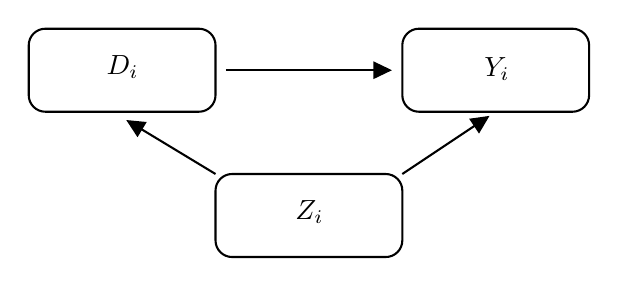
\begin{tikzpicture}[x=0.75pt,y=0.75pt,yscale=-1,xscale=1]
%uncomment if require: \path (0,361); %set diagram left start at 0, and has height of 361

%Rounded Rect [id:dp7232682276583055] 
\draw   (230,168) .. controls (230,163.58) and (233.58,160) .. (238,160) -- (312,160) .. controls (316.42,160) and (320,163.58) .. (320,168) -- (320,192) .. controls (320,196.42) and (316.42,200) .. (312,200) -- (238,200) .. controls (233.58,200) and (230,196.42) .. (230,192) -- cycle ;

%Rounded Rect [id:dp7900793201983274] 
\draw   (320,98) .. controls (320,93.58) and (323.58,90) .. (328,90) -- (402,90) .. controls (406.42,90) and (410,93.58) .. (410,98) -- (410,122) .. controls (410,126.42) and (406.42,130) .. (402,130) -- (328,130) .. controls (323.58,130) and (320,126.42) .. (320,122) -- cycle ;

%Rounded Rect [id:dp49000656757418604] 
\draw   (140,98) .. controls (140,93.58) and (143.58,90) .. (148,90) -- (222,90) .. controls (226.42,90) and (230,93.58) .. (230,98) -- (230,122) .. controls (230,126.42) and (226.42,130) .. (222,130) -- (148,130) .. controls (143.58,130) and (140,126.42) .. (140,122) -- cycle ;

%Straight Lines [id:da16218237230483512] 
\draw    (320,160) -- (359.5,133.66) ;
\draw [shift={(362,132)}, rotate = 146.31] [fill={rgb, 255:red, 0; green, 0; blue, 0 }  ][line width=0.08]  [draw opacity=0] (8.93,-4.29) -- (0,0) -- (8.93,4.29) -- cycle    ;
%Straight Lines [id:da880895933850384] 
\draw    (230,160) -- (189.57,135.55) ;
\draw [shift={(187,134)}, rotate = 31.16] [fill={rgb, 255:red, 0; green, 0; blue, 0 }  ][line width=0.08]  [draw opacity=0] (8.93,-4.29) -- (0,0) -- (8.93,4.29) -- cycle    ;
%Straight Lines [id:da6515543213351532] 
\draw    (235,110) -- (312,110) ;
\draw [shift={(315,110)}, rotate = 180] [fill={rgb, 255:red, 0; green, 0; blue, 0 }  ][line width=0.08]  [draw opacity=0] (8.93,-4.29) -- (0,0) -- (8.93,4.29) -- cycle    ;

% Text Node
\draw (176,101.4) node [anchor=north west][inner sep=0.75pt]    {$D_{i}$};
% Text Node
\draw (267,171.4) node [anchor=north west][inner sep=0.75pt]    {$Z_{i}$};
% Text Node
\draw (358,102.4) node [anchor=north west][inner sep=0.75pt]    {$Y_{i}$};


\end{tikzpicture}
                \caption{Confounders}
                \label{fig:selection/confounders}
            \end{figure}

            How does this relate to selection bias? For example, if the treatment $D_i$ was `health insurance' and outcome variable was `health', then a confounder could be `education'. Education may improve both an individual’s probability of taking health insurance and health outcomes, hence the observed difference is unlikely to be an accurate depiction of the effect of health insurance on health outcomes.


        \subsection{Random assignment}
            Suppose we randomly assign treatment, meaning $Y_{0i}$ and $Y_{1i}$ are independent of $D_i$. From rules of conditional expectation, this means for $j,d\in\{0,1\}$,
            \begin{align}
                \expect{Y_{ji} | D_i = d} = \expect{Y_{ji}}
            \end{align}

            \begin{theorem}
                Under random treatment assignment, the observed difference is equal to the average treatment effect (ATE); that is selection bias is zero.
            \end{theorem}
            \begin{proof}
                Consider the observed difference; due to independence of treatment, we can simplify to
                \begin{align*}
                    \text{observed difference}
                        &:= \expect{Y_{1i}|D_i=1} - \expect{Y_{0i}|D_i=0}   \\
                        &= \expect{Y_{1i}} - \expect{Y_{0i}}    \\
                        &=: \mathrm{ATE}
                \end{align*}
            \end{proof}
            
